\documentclass{ths}
\usepackage{makeidx}
\usepackage{color}
\usepackage{amssymb}
\usepackage{amsmath}
\usepackage{subfigure}
\usepackage{setspace}
\usepackage{graphics}
\usepackage{graphicx}
\usepackage {epsfig}
\usepackage{listings}
\lstset{language=Python}
\usepackage{graphicx}
\usepackage{titlesec}
\usepackage{url}
\usepackage{amsmath}
\usepackage{amssymb}
\usepackage{color}
\usepackage{fancyhdr}
\usepackage {pdfpages}
\documentclass[12pt]{amsart}
\usepackage{geometry}
\usepackage{listings}
\usepackage{color}
\usepackage[usenames,dvipsnames,svgnames,table]{xcolor}
\geometry{a4paper}
\usepackage[T1]{fontenc} 
\usepackage{ae,aecompl}
\usepackage{aeguill}
\usepackage{pslatex}
\usepackage{enumerate}
\usepackage{%
  babel,
  algorithmic,
  algorithm,
  caption
}
\setstretch{1.5}
\usepackage[intoc]{nomencl}
\makeindex
\begin{document}
\title{FINAL-YEAR PROJECT REPORT WRITING GUIDELINES}
\author{NIKHI m wagh}
\date{4 Feb 2013}

\maketitle



\title format{\chapter}
 {\normalfont\large\bfseries\vskip 0cm\headsep 0.2in}{\chaptertitlenames}{16pt}{\large}
\pagenumbering{roman}

\newpage
\centerline{\large{ \textbf{ABSTRACT}}}
\addcontentsline{toc}{chapter}{Abstract}
\vspace{1.5 cm}
Large-scale content-based face image retrieval is an enabling technology for many emerging applications. Existing system ignore strong, face specific geometric constraints among different visual words in a face image. Recent works on face recognition have proposed various discriminative facial features. However, these features are typically high-dimensional and global, thus not suitable for quantization and inverted indexing. There are two orthogonal methods: attribute- enhanced sparse coding and attribute embedded inverted indexing. Attribute-enhanced sparse coding exploits the global structure of feature space and uses several important human attributes combined with low level features to construct semantic code words in the offline stage. On the other hand, attribute-embedded inverted indexing locally considers human attributes of the designated query image in a bi- nary signature and provides efficient retrieval in the online stage. The System may include modules like Content base image search, Attribute base search and Face image retrieval. The proposed System can achieve higher Scalability with Efficient Content Based Image retrieval.
\newline \textbf{Keywords: }
Content-Based Image Retrieval Face Image, Human Attributes, Inverted Indexing

\listoffigures
\addcontentsline{toc}{chapter}{List of Figures}

\listoftables
\addcontentsline{toc}{chapter}{List of Tables}
%---------------------------------------------------------------------

%-------------------------------------------------------------------
\afterpreface
\thispagestyle{empty}
\setcounter{page}{0}
\tableofcontents
\newpage

\pagenumbering{arabic}

\chapter{INTRODUCTION}
\definecolor{gray}{rgb}{0.358411, 0.165, 0.44971}
\lfoot{
\footnotesize{\textcolor{gray}{Topic Name}}}
%\cfoot{``SELECTION OF'' }
%\textcolor{gray}{KKWIEER, Department of Computer Engineering, 2011-2012}
\rfoot{\small{\thepage}}




\section{\normalsize{\textbf{Detailed Problem Definition}}}
The aim of the project is to address one of the important and challenging problems large-scale content-based face image retrieval. Given a query face image, content-based face image retrieval tries to find similar face images from a large image database by detecting facial attributes of given query image. It is an enabling technology for many applications including automatic face annotation, crime investigation.

\section{\normalsize{\textbf{Current Market Survey}}}
Image processing is computer imaging where application involves a human being in the visual loop. In other words the image is to be examined and acted upon by people. Face recognition is not perfect and struggles to perform under certain conditions. Ralph Gross, a researcher at the Carnegie Mellon Robotics Institute, describes one obstacle related to the viewing angle of the face: “Face recognition has been getting pretty good at full frontal faces and 20 degrees off, but as soon as you go towards profile, there have been problems. Other conditions where face recognition does not work well include poor lighting, sunglasses, long hair, or other objects partially covering the subjects face, and low resolution images. Another serious disadvantage is that many systems are less effective if facial expressions vary. Even a big smile can render the system less effective. For in- stance: Canada now allows only neutral facial expressions in passport photos. The need to find a desired face from a collection is shared by many professional groups, including journalists, design engineers and art historians. While the requirements of image users can vary considerably, it can be useful to characterize image queries into three levels of abstraction: primitive features such as shape, logical features such as the identity of objects shown and abstract attributes such as the significance of the scenes depicted. While systems currently operate effectively only at the lowest of these levels, most users demand higher levels of retrieval.

\section{\normalsize{\textbf{Need of the System}}}
Retrieving faces according their attributes from large database is an important task has a wide range of applications such as Crime Investigation, In Medical field, Face detection System. However, retrieving face images from database based on low level attribute is not easy but does not given perfect result. In other words, retrieving face images from database based on low level high level attribute is not easy but gives perfect result with great efficiency than existing system. Traditional methods for face image retrieval usually use low level features to represent faces but low-level features are lack of semantic meanings and face images usually have high intra-class variance (e.g., expression, posing), so the retrieval results are unsatisfactory. To tackle this problem, other proposes to use identity based quantization Chenetal.Propose to use identity-constrained sparse coding, but these methods might require clean training data and massive human annotations. Using fisher vectors with attributes for large-scale image retrieval, but they use early fusion to combine the attribute scores. Also, they do not take advantages of human attributes because their target is general image retrieval.
\newline \textbf{Major contributions of this work are summarized as follows:} 
Although human attributes have been shown useful on applications related to face images, it is non-trivial to apply it in content-based face image retrieval task due to several reasons. First, human attributes only contain limited dimensions. When there are too many people in the dataset, it loses discriminability because certain people attributes. Second, human attributes are represented as a vector of floating points. It does not work well with developing large-scale indexing methods, and therefore it suffers from slow response and scalability issue when the data size is huge.
 
\section{\normalsize{\textbf{Advances to the previous system}}}
Drawbacks of existing approaches System ignore strong, face specific geometric constraints among different visual words in a face image. Recent works on face recognition have proposed various discriminative facial features. How- ever, these features are typically high-dimensional and global, thus not suitable for quantization and inverted indexing. In other words, using such global features in a retrieval system requires essentially a linear scan of the whole database in order to process a query, which is prohibitive for a web-scale image database.
\newline 
In this work the System proposes two orthogonal methods named attribute-enhanced sparse coding and attribute-embedded inverted indexing. Attribute enhanced sparse coding exploits the global structure of feature space and uses several important human attributes combined with low-level features to construct semantic code words in the off-line stage. On the other hand, attribute-embedded inverted indexing locally considers human attributes of the designated query image in a bi- nary signature and provides efficient retrieval in the on-line stage. By incorporating These two methods, we build a large-scale content-based face image retrieval system by taking advantages of both low-level (appearance) features and high-level (Facial) semantics.

\section{\normalsize{\textbf{Organization of the report}}}
The rest of the report is organized as follows: chapter 2 will do the requirement analysis with product function, project plan and team structure, chapter 3 will does the methodologies used for implementation, chapter 4 will show the modeling and design.

%%% Local Variables: 
%%% mode: latex
%%% TeX-master: "../mainrepUG"
%%% End: 

%\chapter{SYNOPSIS}

\chapter{REQUIREMENT ANALYSIS}

\section{\normalsize{\textbf{Requirement analysis}}} 
\subsection{\normalsize{Product Functions}}
\begin{itemize}
\item Query Image
\item Facial Attributes Detection
\item Sparse Code Generator
\item Binary Signature Generation
\item Inverted Indexing
\item Ranking of Resultant Images for Query Image
\item Space complexity Reduces
\item Better performance
\end{itemize}
\subsection{\normalsize{User Classes and Characteristics}}
\textbf{Crime investigation:} 
The Propose System can be use effectively for Criminals identification. Attribute detection from Query Criminal image will retrieve the corresponding matches for Query Image.
\newline \textbf{Medical:}
Medical science can often make excellent use of technologies from other fields. For example, knowledge from automatic facial recognition can also be used for medical analysis of images of organs.
\subsection{\normalsize{Operating Environment}}
\textbf{Hardware Requirement:}
\begin{itemize}
\item 2.80GHz Intel Pentium Processor (min)
\end{itemize}
\textbf{Software Requirement:}
\begin{itemize}
\item Microsoft Windows X P/7(OS)
\item Microsoft V isual S tudio2010
\end{itemize}
\textbf{Dataset:}
\begin{itemize}
\item LFW
\item PubFig
\end{itemize}
\subsection{\normalsize{Design and Implementation Constraints}}
The Propose System will provide Ranking for Query Image with the use of Inverted Indexing but on the behalf of this constraint for Propose System is:
\begin{itemize}
\item Multiple Faces Image will be Rank According to Face Landmark Detection.
\item Query Image should contain Face.
\end{itemize}
\subsection{\normalsize{User Documentation}}
The product will be deploy along with the user manual for the proper guidance to install the software and the tutorials for effectively using various functions provided by the software.
\newpage
\section{\normalsize{\textbf{Project plan}}}
\begin{figure}[ht!]
	\centering
		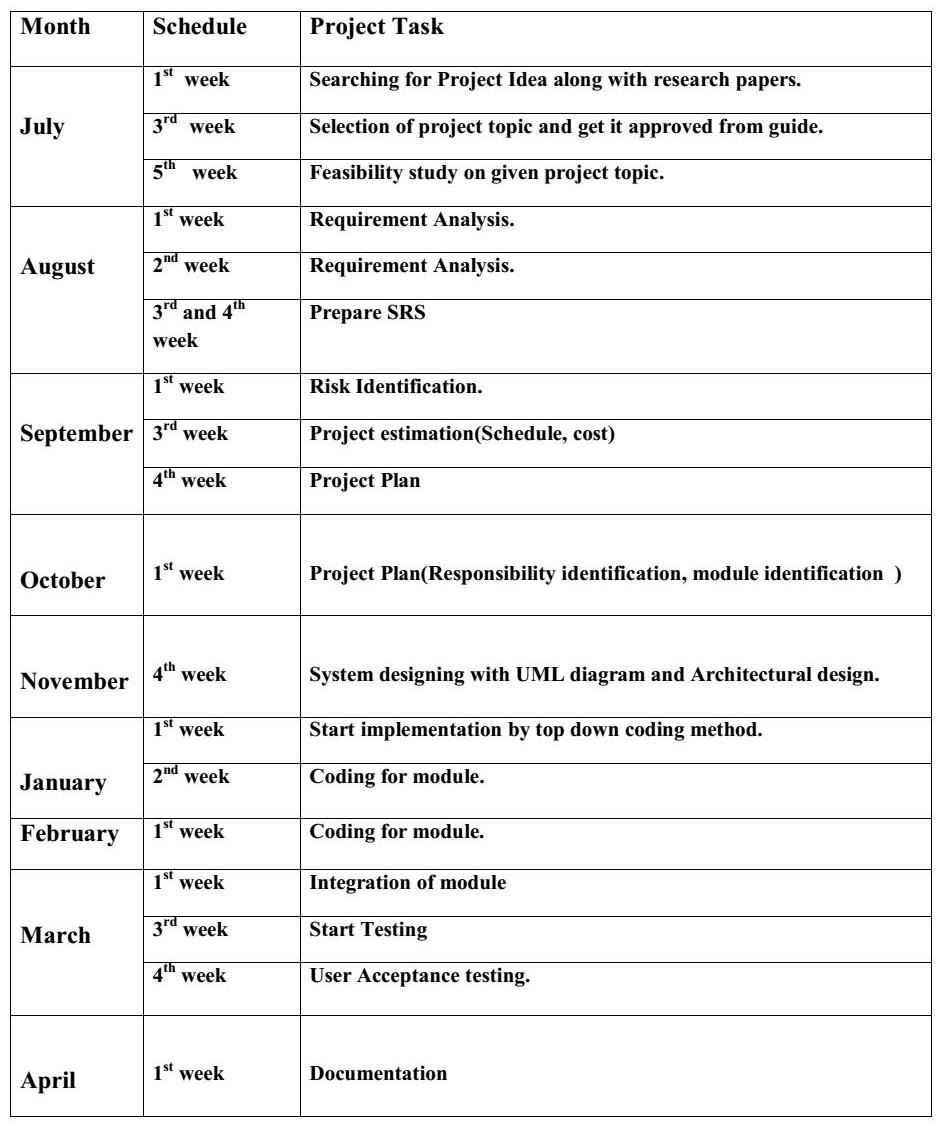
\includegraphics[width=100mm]{plan.jpg}
	\caption{Plan for Project}
	\label{fig:plan}
\end{figure}
\section{\normalsize{\textbf{Team structure}}} 
\begin{table}[h]
\label{sch}
\begin{center}
\begin{tabular}{|c|c|c|c|c|} \hline
		\bfseries Sr.No. & \bfseries Name & \bfseries Task \\ \hline
    \bfseries 1 & Amruta Kumbhakarn &  Coding, Testing \\ \hline
		\bfseries 2 & Sana Mirza &  Documentation, Testing  \\ \hline
		\bfseries 3 & Nikhil Wagh & Coding, Testing  \\ \hline
		\bfseries 4 & Sagar Katarnaware & GUI, Testing  \\ \hline
\end{tabular}
\end{center}
\caption {Team structures.}
\end{table}




%%% Local Variables: 
%%% mode: latex
%%% TeX-master: "../mainrep"
%%% End: 

%\chapter{TECHNICAL KEYWORDS}
\chapter{METHODOLOGY}
\section{\normalsize{\textbf{Softwares used}}}
\begin{itemize}
\item Microsoft Visual Studio 2010
\item Datasets: LFW and PubFig
\end{itemize}
\section{\normalsize{\textbf{Hardware specification}}}
\begin{itemize}
\item Computer with 80GHz Intel Pentium D Processor (min)
\end{itemize}
\section{\normalsize{\textbf{Programming language}}}
\begin{itemize}
\item C\#.net 
\end{itemize}
\section{\normalsize{\textbf{Platform}}}
\begin{itemize}
\item .NET.
\item Windows OS.
\end{itemize}
\section{\normalsize{\textbf{Components}}}
There are four main components in our product given as follows:
\begin{itemize}
\item GUI.
\item Image Files.
\item Attribute Extractor.
\item Sparse Code Generator.
\item Image Raking.
\end{itemize}
\section{\normalsize{\textbf{Tools}}}
Tools used in our product are:
\begin{itemize}
\item Microsoft Visual Studio 2008
\item Microsoft Office 2007
\item Mercury QuickTest Professional 9.2
\end{itemize}
\section{\normalsize{\textbf{Coding style followed}}}
\begin{itemize}
\item Object Oriented Programming.
\end{itemize}

\chapter{MODELING AND DESIGN}
\section{\normalsize{\textbf{UML diagrams and DFDs}}}
\subsection{\normalsize{\textbf{Data Flow Diagrams}}}
\begin{itemize}
\item \textbf {DFD Level 0}
\end{itemize}
\begin{figure}[ht!]
	\centering
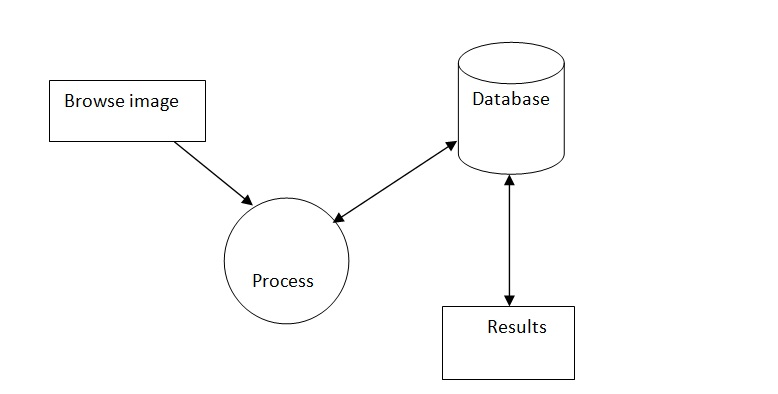
\includegraphics[height=250pt,width=435pt]{dfd0.jpg}\\
\caption{DFD Level-0}
\end{figure}
\newpage
\begin{itemize}
\item \textbf {DFD Level 1}
\end{itemize}
\begin{figure}[ht!]
	\centering
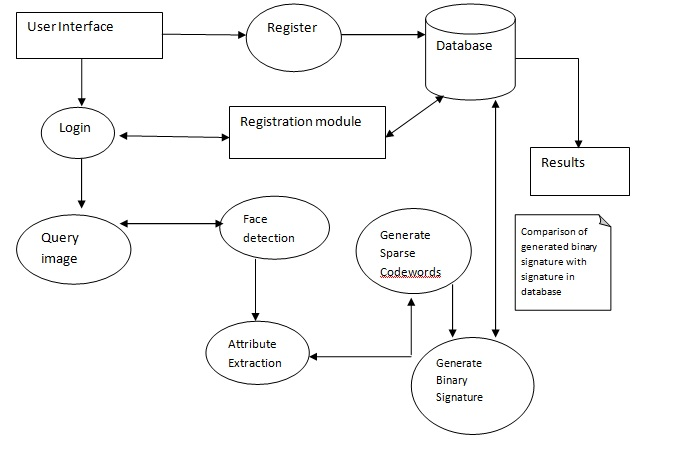
\includegraphics[height=250pt,width=435pt]{dfd1.jpg}\\
\caption{DFD Level-1}
\end{figure}
\subsection{UML Diagrams}
\begin{itemize}
\item \textbf {UseCase Diagram}
\end{itemize}

\begin{figure}[ht!]
	\centering
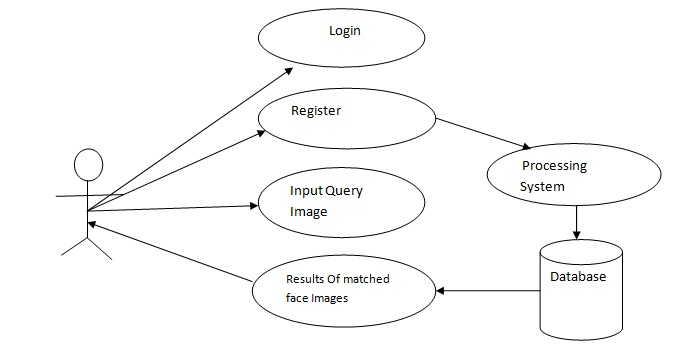
\includegraphics[height=250pt,width=435pt]{usecase.jpg}\\
\caption{UseCase Diagram}
\end{figure}

\newpage
\begin{itemize}
\item \textbf {Class Diagram}
\end{itemize}

\begin{figure}[ht!]
	\centering
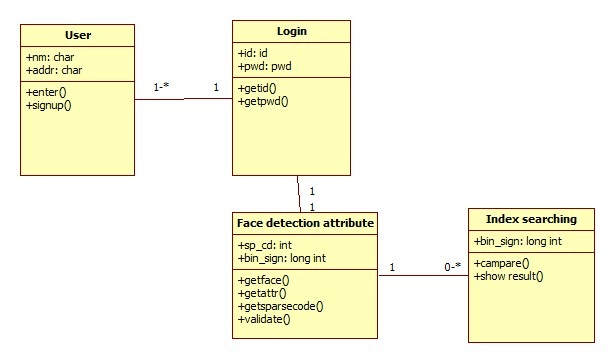
\includegraphics[height=250pt,width=435pt]{class1.jpg}\\
\caption{Class Diagram}
\end{figure}

\begin{itemize}
\item \textbf {Activity Diagram}
\end{itemize}

\begin{figure}[ht!]
	\centering
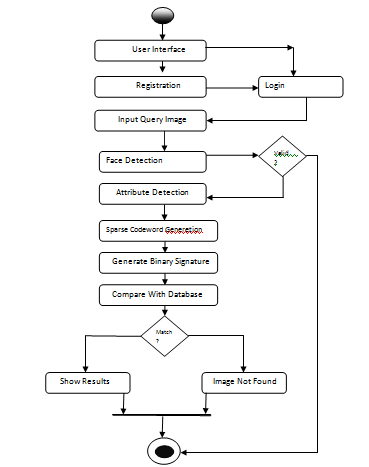
\includegraphics[height=300pt,width=435pt]{acti.png}\\
\caption{Activity Diagram}
\end{figure}
\newline\newline
\begin{itemize}
\item \textbf {Component Diagram}
\end{itemize}

\begin{figure}[ht!]
	\centering
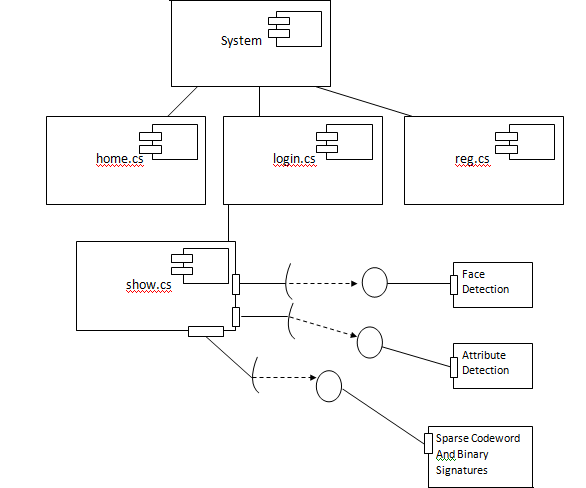
\includegraphics[height=350pt,width=435pt]{comp.png}\\
\caption{Component Diagram}
\end{figure}
\newpage

\begin{itemize}
\item \textbf {Sequence Diagram}
\end{itemize}

\begin{figure}[ht!]
	\centering
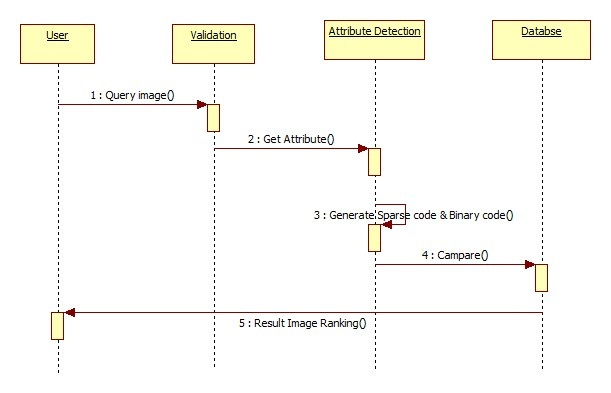
\includegraphics[height=300pt,width=300pt]{Seq.png}\\
\caption{Sequence Diagram}
\end{figure}



\begin{itemize}
\item \textbf {Deployment Diagram}
\end{itemize}

\begin{figure}[ht!]
	\centering
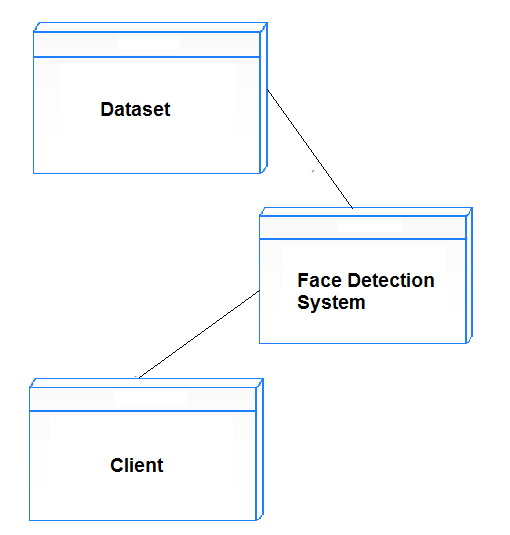
\includegraphics[height=250pt,width=300pt]{dep.png}\\
\caption{Deployment Diagram}
\end{figure}




\section{\normalsize{\textbf{Methods and Procedures}}}
\subsection{\normalsize{\textbf{Modules of the Project}}}
\begin{itemize}
\item \textbf{Face Detection and Attribute Detection:}\newline
This module detects Face from query image by applying Face detection algorithm. We apply another algorithm for attribute detection.
\end{itemize}
\begin{itemize}
\item \textbf{Attribute Enhanced sparse coding:}\newline
This module creates sparse codeword for every Database Image and query image and store for every image in database.
\end{itemize}
\begin{itemize}
\item \textbf{Face Image Retrieval Using Embedded Inverted Indexing:}\newline
This module is used for retrieving images form Database using binary Signature that are generated for every Image in database and Query image using sparse code words. So Indexing is used for Images in database which improves retrieval time and performance of software.
\end{itemize}
\subsection{\normalsize{\textbf{Detailed Flow of the Project}}}
\begin{figure}[ht!]
	\centering
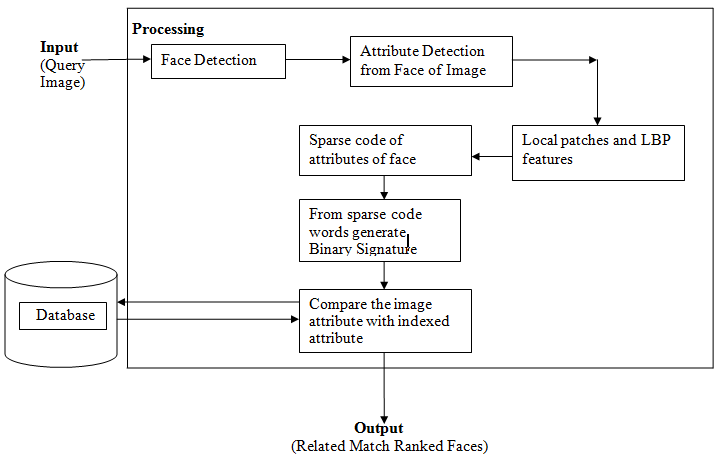
\includegraphics[height=250pt,width=300pt]{block1.png}\\
\caption{Block Diagram}
\end{figure}

\section{\normalsize{\textbf{Screen shots}}}
(decide in consultation with guide)

\chapter{RESULTS}
Results and findings based on the method described in Chapter 4
\begin{table}[ht!]
\caption {Word only result}
\label{tab:Word only result}
\begin{center}
\begin{tabular}{|c|p{2cm}|p{1.5cm}|p{1.5cm}|p{2.1cm}|p{1.5cm}|} \hline

Clustering Method & No. of pages  & No. of cluster & Precision & Recall & F-Measures \\ \hline 

Word  only & 5 & 	3 & 0.6666  &	0.4000 & 49.80  \\ \hline 
&10 & 3& 0.6666 & 0.4000 & 49.80  \\ \hline 
 & 15 & 3 & 0.4444. & 0.2600 & 32.60  \\ \hline 
&15	&4		&0.5555	&0.3333	&42.04 \\ \hline 

\end{tabular}
\end{center}
\end{table}
\chapter{TESTING}
\begin{itemize}
\item \textbf {Test Cases (Manual Testing):}
\end{itemize}

\begin{figure}[ht!]
	\centering
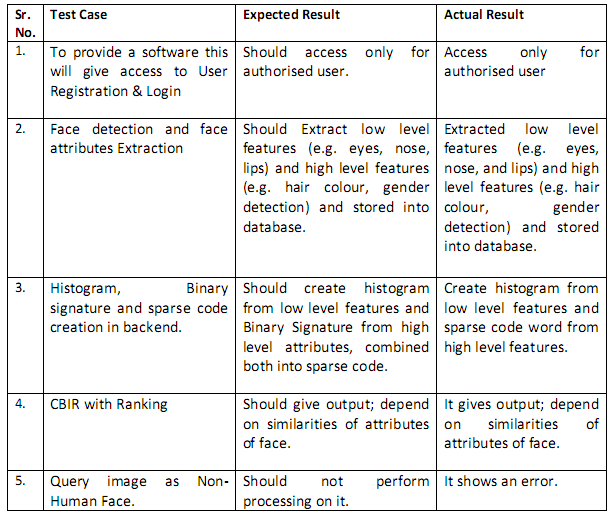
\includegraphics[height=250pt,width=450pt]{test.png}\\
\caption{Test Cases}
\end{figure}
\begin{itemize}
\item \textbf {Testing by Automation Tool:}
\end{itemize}
 We used MERCURY\'s Quick Test Professional 9.2 automation tool for testing our project, we choose this tool because it\’s very efficient for testing and worldwide accepted for testing. QTP can perform following types of testing:\newline\newline\newline\newline
1.	GUI Testing.\newline
2.	Data Driven Testing\newline
3.	Accessibility Testing\newline
4.	Text and Text Area Testing\newline
\textbf{Reasons for choosing QTP for test Automation:}\newline
1.Test Automation framework: From a test framework perspective QTP is one tool that can be used in any type of framework Modular (Record and Playback) driven framework, Data driven (Data tables) Framework (Wow! I love the built in data driver functions and the data driving capabilities of QTP, simply amazing!!!),Keyword driven (Keyword view, function libraries etc.) framework or any other custom framework.\newline
2. Record and Playback: It is pretty easy even for a non-programmer to record scripts / test cases, customize / modify and play back the tests. Also the tool lets the user record the scripts in three different recording modes as per the requirement: Normal, Analog and Low level. Unlike other tools that records every mouse / keyboard events / any java script event on the application, QTP Normal recording mode knows what to record and what not to. The best part is, if you want to record the above said events it can be achieved through the other two recording modes in QTP.\newline
3. Object repository and Object identification process: The Object repository again available in two modes (Shared-For common application objects and Local-For script specific application objects) is personally the best thing I like about QTP. Unlike Test Complete (where a complex object mapping concept is followed), QTP stores the standard and nonstandard properties of the various objects of the AUT (Application under test). At the time of execution, QTP knows exactly where the objects are and how to reach those in a jiffy which increases the efficiency of test execution. The smart processing QTP is definitely a feather on the hat. There is also an ‘object spy’ tool that help you chose the property of an object you can use to automate.\newline
4. In-built function libraries: Quick test professional comes with a huge list of in-built functions (VBScript/QTP) for data manipulation, math, date and time, conversion, string, join and many more functions are available. This ensures that we don’t have to re-invent the wheel, just use it.\newline 
5. Error-Root cause analysis and Recovery: As a tester, I would look for 2 primary things in any application 1: Proper and appropriate error messages 2: Good log reports. Fortunately, Quick Test professional comes with both. Apart from the logs and error messages, we can set break points and find out the values stored in variables at runtime through the full featured Script editor and script debugging features. The recovery scenario manager helps you to recover from any unforeseen events like object state not identified, pop-ups, a statement failure, application crash etc.\newline 
6. Maintenance and Reusability: The idea behind any test automation framework is either Maintainability or Reusability or both. Quick Test professional makes it even easier to maintain the Test Scripts, Functions, objects and everything else built using QTP.\newline
7. Supported environments: Though the tool supports only Windows platform, it can be used for automation in a big list of application platforms but not limited to Java, Oracle, SAP, .NET, Web Forms, Siebel, PeopleSoft, Web services, Main frame (Terminal Emulator), Stingray, Delphi, WPF, Flex, Windows mobiles and not to forget the support for most popular browsers like Internet explorer and fire fox. From the forums, I understand that they are working on support for Google chrome browser. It also supports Rich Internet Applications (RIA) like Ajax, Flex, Silverlight, etc.\newline
8. Support for different testing requirements: Quick Test professional supports any level of testing (Unit, Integration, System, and UAT), regression testing, web application testing, windows application testing, mobile application testing, database, load testing etc. Please read the complete article on QTP supported testing types by clicking on the link.\newline
9. Results viewer: The test run Results viewer furnishes with an executive summary page with data specific to the test , pie charts and statistics for both the current and previous runs, a quick link to the previous run results, and more. It is pretty easy to customize or the set of panes that we can show, hide, move, dock. The best part is the Run results viewer can be installed as a standalone application. This enables us to share the results of the tests with business analysts and developers who do not work with Quick Test professional.\newline
\textbf {We used QTP 9.2 for GUI and Accessibility Testing}

\newpage
\textbf{Snapshot of QTP Testing:}

\begin{figure}[ht!]
	\centering
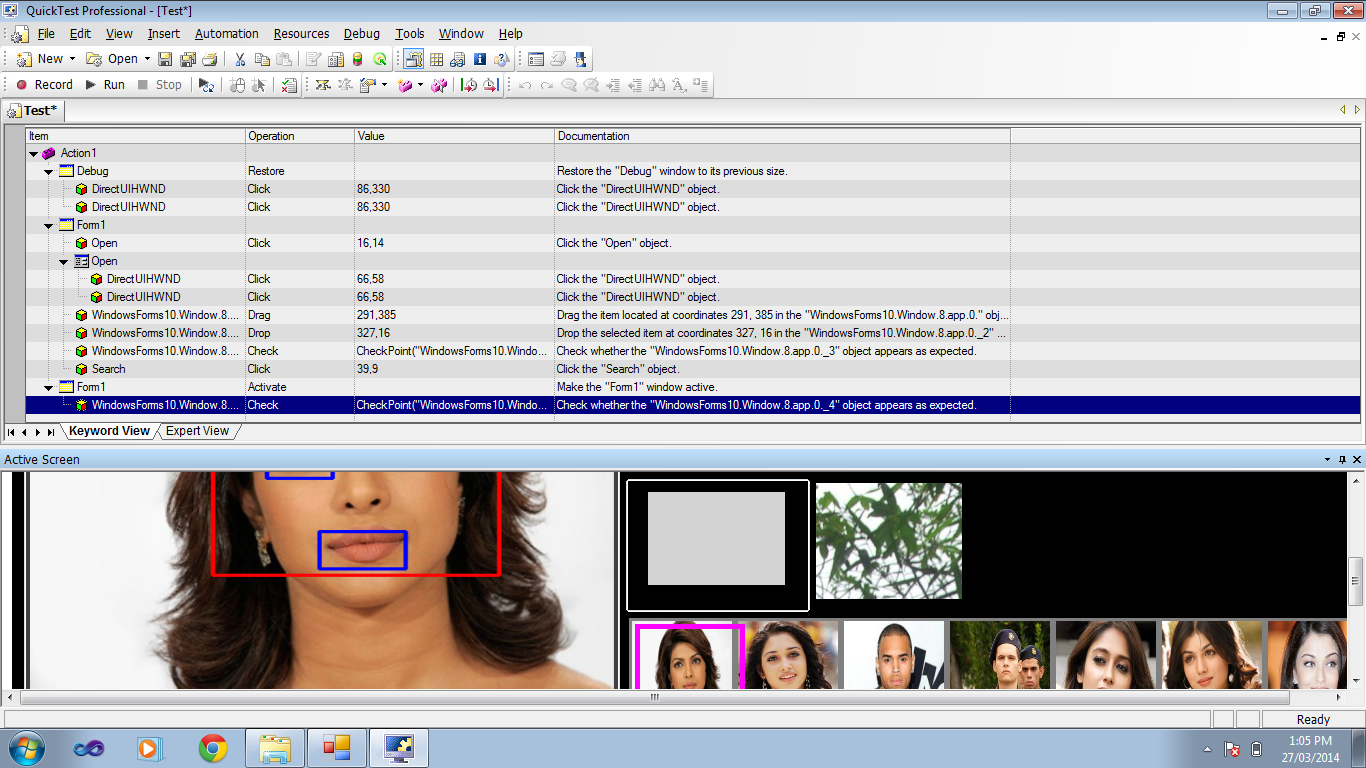
\includegraphics[height=250pt,width=450pt]{qtp1.png}\\
\caption{BitMap Checkpoints in QTP}
\end{figure}

\begin{figure}[ht!]
	\centering
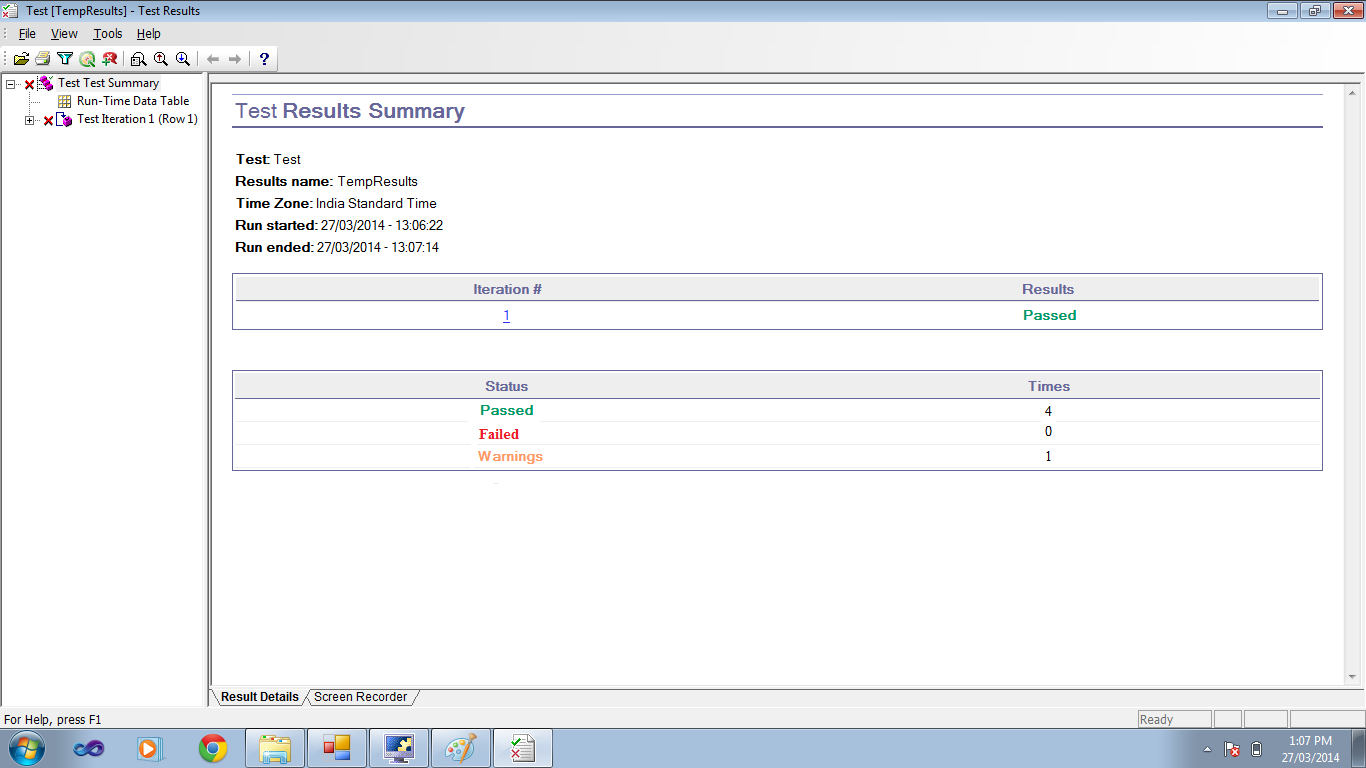
\includegraphics[height=250pt,width=450pt]{test_result.png}\\
\caption{Test Result}
\end{figure}


\appendix
\chapter{Appendix A}
\input{chapter_A}
\chapter{Appendix B}
\input{chapter_B}
\end{appendix}
\newpage
\prefacesection{Bibliography}
%s\bibliographystyle{IEEEtran}

%\begin{thebibliography}{1}
\begin{enumerate}
\item Ando, R. K., and Zhang, T. Two-view feature generation model for semi-supervised learning. In ICML '07 (2007)\\
\item AnusuaTrivedi, PiyushRai, Scott L. DuVall "Exploiting Tag and Word  Correlations for Improved Webpages Clustering "SMUC'10, October 30,2010, Toronto, Ontario, Canada. Copyright 2010 ACM.

\item AntonelaTommasel and Daniela Godoy, "Semantic enrichment of social annotations for Webresource classification"JAIIO - ASAI 2012
\item ArkaitzZubiaga, Raquel Mart�nez,V�ctor Fresno "Getting the Most Out of Social Annotations for Web PageClassification"Document Engineering, pages 74-83 , 2009.
\end{enumerate}

\prefacesection{Acknowledgement}
 With Deep Sense of Gratitude, We would like to Thanks all the People who have lit our path with their kind guidance. We are very Grateful to those intellectuals who did their best to help during our Project work for this semester. It is our proud privilege to express deep sense of gratitude to, Prof.S.S.Sane Sir for his comments and kind permission to complete this project work for this Semester We remain indebted to Project Coordinator Prof. and Project Guide Prof.S.S.Bhandare for their timely suggestion and valuable guidance. The special gratitude goes to all the staff members, technical staff members, of computer engineering department for their expensive, excellent and precious guidance in completion of this work. We thank to all the colleagues for their appreciable for our working project.	
%-----------------------------------------abhorase
%\bibliographystyle{IEEEtran}
%\bibliographystyle{plain}
%s\bibliography{gkp2}
\end{document} 